\documentclass{report}
\usepackage[utf8]{inputenc}
\usepackage[top=1cm, bottom=2cm, left=2cm, right=2cm]{geometry}
\usepackage[francais]{babel}
\usepackage[T1]{fontenc}
\usepackage{graphicx}
\usepackage{subcaption}
\usepackage{listings}
\usepackage{hyperref}
\usepackage{wrapfig}

\title{Rapport}
\author{François PIAT}
\date{WEEK 8}

\begin{document}

\maketitle

\chapter*{Profiling}
- Tests sur "Register" très long pour le modèle FFD.\\
- A la fin de la semaine, on a pu interpréter les résultats du modèle Rigid et Affine avec et sans l'action de TBB. 
Les résultats montrent sur (sur ces 2 modèles), des performances améliorées d'un taux de 4x quand TBB est actif. Les résultats complets apparaîtront dans le prochain rapport.

\chapter*{Implémentation}	

\paragraph{Stratégie}
On s'intéresse à l'implémentation avec ArrayFire de "GaussianBlurring" utilisé pour la fonction "smooth-image". La fonction actuelle s'articule tel que suit.
\begin{lstlisting}
Initialisation:

Run:
- Recuperation de la matrice a traiter
- Blurring sur la dimension 1
	- Initialisation du kernel (kernel = filtre)
	- Produit de convolution entre la matrice d'entree et le filtre
- Blurring sur la dimension 2 (Implementation idem que 1)
- Blurring sur la dimension 3 (Implementation idem que 1)
- Blurring sur la dimension 4 (Implementation idem que 1)
- Retour en sortie de la matrice filtree

Finalisation:
\end{lstlisting}
- On peut remarquer que l'implémentation des filtres est séparable, c'est-à-dire que chaque dimension déclare son propre kernel sur une dimension, puis éxecute la convolution sur cette même dimension. En revanche,  avec Arrayfire, la stratégie sera de préparer un kernel au fur et à mesure qu'on l'étudie sur chaque dimension, puis de le convoluer directement à la matrice d'entrée globale en fin de fonction.
\\
\\
- On décide de ne pas s'intéresser à la dimension temporelle (4D) pour le moment.\\
\\
- Dans un premier temps, on a abordé le problème de la sorte :

\begin{figure}[h!]
	\begin{center}
		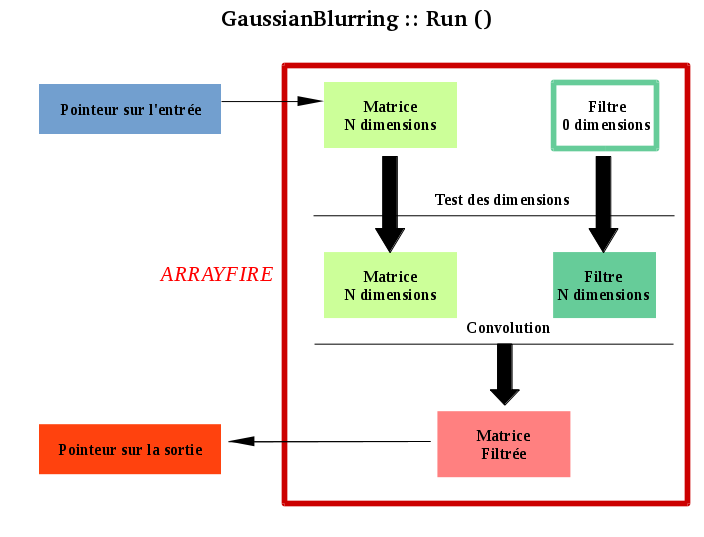
\includegraphics[height=8cm]{figures/gaussianblurring.png}
		\caption{Architecture de la fonction de flou gaussien - Implémentation des filtres non-séparables}
		\label{Architecture de la fonction de flou gaussien - Implémentation des filtres non-séparables}
	\end{center}
\end{figure}

Contrairement à l'implémentation MIRTK, on analyse ici chaque dimension de la matrice, adapte le kernel, et opère une seule convolution une fois le kernel préparé.\\
Cependant, ArrayFire ne permettant pas de broadcasting, on n'a pas pu procéder de la sorte, on a directement utilisé un algorithme plus optimisé, qui consiste à convoluer chaque dimension l'une après l'autre, en arrangeant la matrice à chaque fois. (cf Résultats)
\paragraph{Résultats}
La fonction finale est implémentée de la sorte :
\begin{figure}[h!]
	\begin{center}
		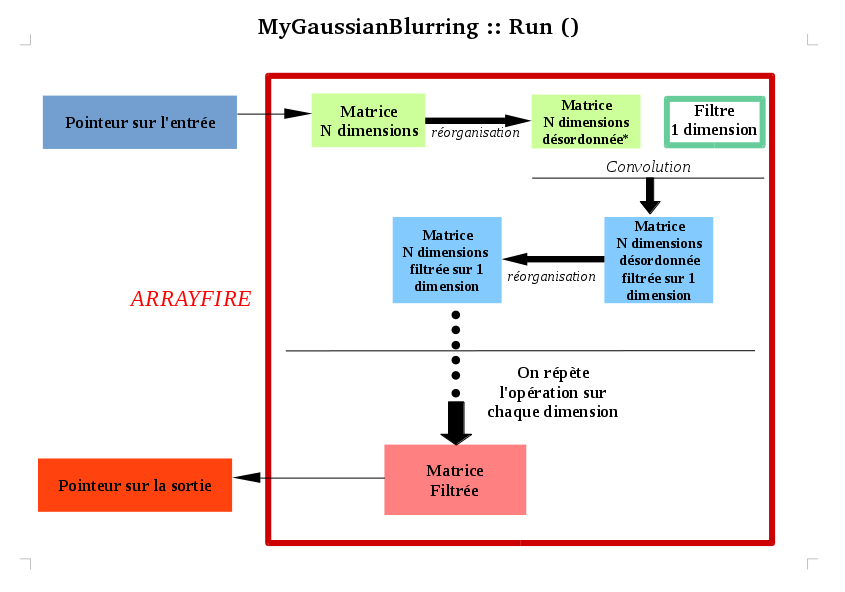
\includegraphics[height=10cm]{figures/mygaussianblurring.png}
		\caption{Architecture de la fonction final de flou gaussien - Implémentation des filtres séparables}
		\label{Architecture de la fonction finale de flou gaussien - Implémentation des filtres séparables}
	\end{center}
\end{figure}
\\
**: la réorganisation de la matrice est nécessaire pour réaliser la convolution en 1 seule dimension. Si, par exemple, on veut convoluer la matrice sur l'axe Z, il faut au préalable inverser les axes X et Z (puisque X est défini comme le 1er axe et que la convolution s'appliquera sur celui-ci). 
\paragraph{Problèmes}
L'API d'ArrayFire permet de couvrir la majorité des pré-requis de la fonction "GaussianBlurring", excepté la génération d'un kernel Gaussien 3D et les produits de convolution séparés. \\
\\
- Les produits de convolution étant séparables (afin de distinguer différentes intensité de floutage sur chaque dimension => exemple : faible floutage sur la profondeur, mais important sur la hauteur), il a fallu trouver un moyen de reproduire ce même calcul avec ArrayFire.\\
Dans un premier temps, on se satisfera d'une convolution directe en 3 dimensions, en créant un kernel 4D qui aura les mêmes dimensions que désirées (exemple, kernel de dimension[X,Y,1,1] si on veut étudier une image 2D).\\
\\
- Une déclaration MIRTK (qui fournit les dimensions des matrices, sous forme d'attributs) ET une déclaration ArrayFire sont indispensables pour utiliser ArrayFire dans les opérations qui suivent => 2 déclarations : pas optimal. Cependant, pour utiliser ArrayFire, il est inévitable de déclarer un type "GenericImage", afin d'obtenir ses dimensions.
\\
\\
- Le setup d'un nouveau projet, appelant simplement une classe dérivée d'une classe de MIRTK a été compliqué à mettre en place. C'est à partir de ce projet que l'on commence l'implémentation de la fonction \textbf{"GaussianBlurring"} avec ArrayFire. Les écritures préalables faisant office de brouillons.

\chapter*{Bazar}
Article bien expliqué concernant le principe du traitement d'image à base de convolution de matrices : \\ 
\url{https://docs.gimp.org/en/plug-in-convmatrix.html}



\end{document}